%!TEX root = ../func_top.tex

\section{Existence of persistence diagrams} \label{s:connectivity}

We have seen that q-tame functions admit persistence diagrams, which can be used to formulate Morse inequalities.
With q-tameness being a rather abstract algebraic property, we now establish concrete topological conditions that ensure the q-tameness of a function.
Our definitions are motivated by similar conditions considered by Morse in his work on functional topology.
We will present a historical account in \cref{s:surfaces}.

Whether a function is q-tame or not depends on the functor that is used to pass from the sublevel set filtration of the function to a persistence module.
The general strategy is to deduce global finiteness properties like q-tameness from local ones.
Thus, the functors we consider should have a certain property allowing us to do so.

Specifically, let $\H = (\H_d)_{d \in \Z} \colon \Top \to \Vect$ be a fixed graded homotopy invariant functor, which we call a \emph{homology theory}.
A triple of spaces $X_{1}, X_{2} \subseteq X$ is said to have a \emph{Mayer--Vietoris sequence} for $\H$ if the inclusion-induced maps can be completed to a long exact sequence
\begin{equation*}
\begin{tikzcd}[column sep = small]
\cdots \arrow[r] &[-10pt] \H_{n+1}(X) \arrow[d] & &[-20pt] & \\
& \H_{n}(X_{1} \cap X_{2}) \arrow[r] &
\H_{n}(X_{1}) \oplus \H_{n}(X_{2}) \arrow[r] &
\H_{n}(X) \arrow[d] \\ & & &
\H_{n-1}(X_{1} \cap X_{2}) \arrow[r] &
\cdots \ .
\end{tikzcd}
\end{equation*}
We say that $\H$ has the \emph{open} (resp.\@\ \emph{compact}) \emph{Mayer--Vietoris property} if there are natural Mayer--Vietoris sequences for all triples $X_{1}, X_{2} \subseteq X$ with $X = X_1 \cup X_2$ and $X_i \subseteq X$ open (resp.\@\ compact Hausdorff).

For the rest of this section, we will assume that $\H$ is a homology theory that has either the open or the compact Mayer--Vietoris property and for which there is $n_0$ such that $\H_{n}$ is zero for all $n \leq n_0$.
We will also assume that $\H_{n}$ takes finite dimensional values on one-point spaces.
Note that this includes singular homology with field coefficients, which has the open Mayer--Vietoris property (like any homology theory in the sense of the Eilenberg--Steenrod axioms \cite[Chapter I]{Eilenberg.1952}), and it also includes \v{C}ech homology with field coefficients, which has the compact Mayer--Vietoris property by \cite[Theorem 10.7.2]{tomDieck.2008} as a consequence of the strong excision property of \v{C}ech homology \cite[Theorem X.5.4]{Eilenberg.1952}.

\subsection{Local connectivity and q-tameness}

\begin{defi}
	For $n \in \Z$, a continuous map is said to be \emph{$n$-homologically small} or $\HS_n$ if the image of the map induced by $\H_{n}$ is finite dimensional.
	We omit references to $n$ if the condition holds for all integers.
\end{defi}

\begin{defi}
	The sublevel set filtration of a function $f \colon X \to \R$ is called \emph{locally homologically small} or \emph{$\HLC$} if for any $x \in X$, any neighborhood $V$ of $x$, and any pair of indices $s,t$ with $f(x) < s < t$ there is a neighborhood $U$ of $x$ with $U \subseteq V$ such that the inclusion $f_{\leq s} \cap U \hookrightarrow f_{\leq t} \cap V$ is $\HS$.
\end{defi}

\begin{defi}
	We say that a sublevel set filtration is \emph{compact} if all sublevel sets are compact Hausdorff spaces.
\end{defi}

If $f_{\leq t}$ is compact for all $t$, then the function $f$ is necessarily lower-semicontinuous and bounded from below (see \cite[p.~444]{Morse.1939} or \cite[Theorem 3.1]{Struwe.1988}).

Our main result, proven in the remainder of this subsection, is that for compact sublevel set filtrations the $\HLC$ condition implies \mbox{q-tameness}, and consequently also the existence of a persistence diagram:

\begin{thm} \label{t:local connectedness implies q-tameness}
	If the sublevel set filtration of a function $f \colon X \to \R$ is compact and	$\HLC$, then its persistent homology is also q-tame.
	In particular, $f$ has a persistence diagram.
\end{thm}

The general proof strategy is inspired by the proof of Wilder's Finiteness Theorem \cite[p.~325]{Wilder.1949} as presented by Bredon \cite[Section II.17]{Bredon.1997}.
We collect the main ideas in several lemmas.

\begin{lem} \label{l:commutative algebra}
	Given a commutative diagram of modules over a principal ideal domain
	\begin{equation*}
	\begin{tikzcd}
	A_{1,1} \arrow[r] & A_{1,2} & \\
	A_{2,1} \arrow[r] \arrow[u] & A_{2,2} \arrow[r] \arrow[u] & A_{2,3} \\
	& A_{3,2} \arrow[r] \arrow[u] & A_{3,3} \arrow[u]
	\end{tikzcd}
	\end{equation*}
	where the middle row is exact and both $A_{2,1} \to A_{1,1}$ and $A_{3,3} \to A_{2,3}$ have finitely generated images, then so does $A_{3,2} \to A_{1,2}$.
\end{lem}

\begin{proof}
	This is proven via a straightforward diagram chase.
	For more details see \cite[Lemma II.17.3]{Bredon.1997}.
\end{proof}

\begin{lem} \label{l:neighborhood third}
	Let $X$ be a locally compact Hausdorff space.
	For any compact subset~$K$ and open set $U$ with $K \subseteq U$ there exists a compact set $K^\prime$ such that
	\begin{equation*}
	K \subseteq \interior(K^\prime) \subseteq K^\prime \subseteq U.
	\end{equation*}
\end{lem}

\begin{proof}
	For any $x \in K$ choose a compact neighborhood $C(x) \subseteq U$.
	We have
	\begin{equation*}
	K \subseteq \bigcup_{x \in K} \interior(C(x)).
	\end{equation*}
	Since $K$ is compact, there is a finite subset $\{x_1, \dots, x_m\}$ of elements in $K$ so that
	\begin{equation*}
	K \subseteq \bigcup_{i=1}^m \interior(C(x_i)) \subseteq \interior\left(\bigcup_{i=1}^m C(x_i)\right) \subseteq \bigcup_{i=1}^m C(x_i) \subseteq U
	\end{equation*}
	Defining $K^\prime = \bigcup_{i=1}^m C(x_i)$ finishes the proof.
\end{proof}

We want to use \cref{l:neighborhood third} on the domain of the function whose sublevel set filtration we consider.
However, we do not want to assume the domain to be locally compact for \cref{t:local connectedness implies q-tameness}.
To circumvent this, we will work in one of the sublevel sets, which are assumed to be compact Hausdorff and hence locally compact.
This requires the use of a slight weakening of the $\HLC$ condition.

\begin{defi}
	For $u \in \R$, the sublevel set filtration of a function $f \colon X \to \R$ is called \emph{$\HLC$ below $u$} if, for any $x \in X$, any neighborhood $V$ of $x$, and any pair of indices $s,t$ with $f(x) < s < t < u$, there is a neighborhood $U$ of $x$ with $U \subseteq V$ such that the inclusion $f_{\leq s} \cap U \hookrightarrow f_{\leq t} \cap V$ is $\HS$.
\end{defi}

\begin{lem} \label{l:restriction of LHS filtration}
	Let $f \colon X \to \R$ be a function whose sublevel set filtration is $\HLC$.
	Fix $u \in \R$ and let $g \colon Y \to \R$ be the restriction of $f$ to the sublevel set $Y = f_{\leq u}$.
	Then the sublevel set filtration defined by $g$ is $\HLC$ below $u$.
\end{lem}

\begin{proof}
	Let $x \in Y$, let $V$ be a neighborhood of $x$ in $Y$, and consider indices $s,t$ with $g(x) < s < t < u$.
	We need to find a neighborhood $U \subseteq V$ of $x$ such that the inclusion $g_{\leq s} \cap U \hookrightarrow g_{\leq t} \cap V$ is $\HS$.

	Since $Y \subseteq X$ carries the subspace topology, we may choose a neighborhood $V'$ of $x$ in $X$ such that $V = V' \cap Y$.
	The sublevel set filtration of $f$ is assumed to be $\HLC$, so there is a neighborhood $U' \subseteq V'$ of $x$ in $X$ such that the inclusion $f_{\leq s} \cap U' \hookrightarrow f_{\leq t} \cap V'$ is $\HS$.
	We set $U = U' \cap Y$, which defines a neighborhood of $x$ in $Y$.

	Now $s < t < u$ implies that $g_{\leq s} = f_{\leq s}$ and $g_{\leq t} = f_{\leq t}$.
	Moreover, we have $f_{\leq s} \cap Y = f_{\leq s} \cap f_{\leq u} = f_{\leq s}$ and $f_{\leq t} \cap Y = f_{\leq t} \cap f_{\leq u} = f_{\leq t}$.
	Thus, we obtain $g_{\leq s} \cap U = f_{\leq s} \cap Y \cap U' = f_{\leq s} \cap U'$ and $g_{\leq t} \cap V = f_{\leq t} \cap Y \cap V' = f_{\leq t} \cap V'$.
	This implies that the inclusion $g_{\leq s} \cap U \hookrightarrow g_{\leq t} \cap V$ is $\HS$ because it agrees with the inclusion $f_{\leq s} \cap U' \hookrightarrow f_{\leq t} \cap V'$, which is $\HS$ by assumption.
	This finishes the proof.
\end{proof}

\begin{lem} \label{l:key lemma for q-tameness}
	Let $f \colon Y \to \R$ be a function on a locally compact Hausdorff space~$Y$ whose sublevel set filtration is compact and $\HLC$ below $u \in \R$, and consider subsets $C \subseteq L \subseteq Y$ with $C$ compact and $L$ open.
	For any $s < t < u$ the inclusion $C \cap f_{\leq s} \hookrightarrow L \cap f_{\leq t}$ is $\HS$.
\end{lem}

\begin{proof}
	Recall our assumption that the underlying homology theory $\H$ has either the open or the compact Mayer--Vietoris property and that there is some $n_0$ such that $\H_{n}$ is zero for all $n \leq n_0$.
	The statement of the lemma holds for $\HS_{n}$ in place of $\HS$ for any $n \leq n_0$ since $\H_{n}$ induces the zero map.
	We will proceed by induction on $n \geq n_0$ assuming the statement for $\HS_{n-1}$.

	We define $\Sigma_{s, t}$ to be the collection of all open subsets $V \subseteq Y$ whose closure $\overline{V}$ is compact, contained in $L$, and has an open neighborhood $U$ with $\overline{V} \subseteq U \subseteq L$	for which there exists $s' \in (s,\, t)$ such that the inclusion $U \cap f_{\leq s'} \hookrightarrow L \cap f_{\leq t}$ is $\HS_n$.
	We will show that $\Sigma_{s, t}$ has the following two properties:
	\begin{enumerate}
		\item Any point $x \in L \cap f_{\leq s}$ has a neighborhood $V_x \in \Sigma_{s,t}$.
		\item If $V_1,\, V_2 \in \Sigma_{s,t}$ then $V_1 \cup V_2 \in \Sigma_{s,t}$.
%		\item For each $V \in \Sigma_{s,t}$ the inclusion
%		$V \cap f_{\leq s} \hookrightarrow L \cap f_{\leq t}$ is $\HS_n$.
	\end{enumerate}

	Assuming them for the moment, the first property allows us to cover $C \cap f_{\leq s}$ by sets $V_x \in \Sigma_{s,t}$, $x \in C \cap f_{\leq s}$.
	Because both $C$ and $f_{\leq s}$ are compact, $C \cap f_{\leq s}$ is again compact, and hence the cover can be chosen finite, represented by say $x_1,\dots, x_m$.
	By the second property, we have
	\[V \defeq \bigcup_{i = 1}^m V_{x_i} \in \Sigma_{s,t}.\]
	Thus, there exists an open neighborhood $U$ of $\overline{V}$ in $L$ and $s' \in (s,\, t)$ such that the inclusion
	$U \cap f_{\leq s'} \hookrightarrow L \cap f_{\leq t}$
	is $\HS_n$.
	The inclusion
	$C \cap f_{\leq s} \hookrightarrow L \cap f_{\leq t}$
	factors through the previous one, so it is $\HS_n$ as well.
	What is left to do is to show that $\Sigma_{s,t}$ has the two claimed properties.


	Next, we will show using the $\HLC$ property that $\Sigma_{s, t}$ has the first required property, i.e., that any point $x \in L \cap f_{\leq s}$ has a neighborhood in $\Sigma_{s, t}$.
	Choose an arbitrary $s' \in (s,\, t)$.
	Since the sublevel set filtration of $f$ is $\HLC$ below $u$ and we have $f(x) \leq s < s' < t < u$, there is an open neighborhood $U_x \subseteq L$ such that the inclusion
	$U_x \cap f_{\leq s'} \hookrightarrow L \cap f_{\leq t}$
	is $\HS$, so in particular $\HS_n$.
	By local compactness of $Y$ we can choose a compact neighborhood $K_x$ of $x$ contained in $U_x$.
	Now $V_x = \interior (K_x)$ is a neighborhood of $x$ with $V_x \in \Sigma_{s,t}$.

	Finally, using the Mayer--Vietoris property and the induction hypothesis we will show that $\Sigma_{s,t}$ has the second required property, i.e., that it is closed under finite unions.
	So for $i \in \{1, 2\}$ let $V_i \in \Sigma_{s,t}$ with $U_i$ and $s'_i \in (s,\, t)$ such that
	$\overline{V_i} \subseteq U_i \subseteq L$
	and
	$U_{i} \cap f_{\leq s'_i} \hookrightarrow L \cap f_{\leq t}$
	is $\HS_n$.
	Writing $K_i = \overline{V_i}$, we use \cref{l:neighborhood third} to construct compact sets $K'_i$ such that
	\begin{equation*}
	V_i \subseteq K_i \subseteq V'_i \subseteq K'_i \subseteq U_i \subseteq L
	\end{equation*}
	where $V'_i = \interior(K'_i)$.
	The union $V_1 \cup V_2 \subseteq L$ is open, its closure $\overline{V_1 \cup V_2}$ is compact, and $\overline{V_1 \cup V_2} \subseteq V'_1 \cup V'_2 \subseteq L$.
	Thus, we obtain $V_1 \cup V_2 \in \Sigma_{s,t}$ if we can show that there is an $s' \in (s,\, t)$ such that the inclusion
	$\left(V'_1 \cup V'_2 \right) \cap f_{\leq s'} \hookrightarrow L \cap f_{\leq t}$
	is $\HS_n$.
	To do so, we set $s'' = \min_i s'_i$ and choose $s' \in (s,\, s'')$.
	For proving that $\left(V'_1 \cup V'_2 \right) \cap f_{\leq s'} \hookrightarrow L \cap f_{\leq t}$ is $\HS_n$ we now distinguish the two cases where $\H$ has either the open or the compact Mayer--Vietoris property.

	For the open Mayer--Vietoris property, note that for both $i \in \{1, 2\}$ the inclusions
	$U_i \cap f_{\leq s''} \hookrightarrow L \cap f_{\leq t}$
	are $\HS_n$.
	Moreover, the inclusion
	$V'_1 \cap V'_2 \cap f_{\leq s'} \hookrightarrow U_1 \cap U_2 \cap f_{\leq s''}$
	is $\HS_{n-1}$ because it factors through the inclusion
	$K'_1 \cap K'_2 \cap f_{\leq s'} \hookrightarrow U_1 \cap U_2 \cap f_{\leq s''}$,
	which is $\HS_{n-1}$ by the induction hypothesis.
	Because the $V_i$ and $V'_i$ are open and because $\H$ has the open Mayer--Vietoris property, we obtain the following commutative diagram satisfying the assumptions of \cref{l:commutative algebra}:
	\[
	\begin{tikzcd}[column sep=small,every matrix/.append style={nodes={font=\small}}]
	\H_n(L \cap f_{\leq t}) \oplus \H_n(L \cap f_{\leq t}) \arrow[r] &
	\H_n(L \cap f_{\leq t}) & \\
	\H_{n}(U_1 \cap f_{\leq s''}) \oplus \H_n(U_2 \cap f_{\leq s''}) \arrow[r] \arrow[u] &
	\H_{n}((U_1 \cup U_2) \cap f_{\leq s''}) \arrow[r] \arrow[u] &
	\H_{n-1}(U_1 \cap U_2 \cap f_{\leq s''}) \\ &
	\H_{n}((V'_1 \cup V'_2) \cap f_{\leq s'}) \arrow[r] \arrow[u] &
	\H_{n-1}(V'_1 \cap V'_2 \cap f_{\leq s'}) \arrow[u].
	\end{tikzcd}
	\]
	We conclude that the inclusion
	$\left(V'_1 \cup V'_2 \right) \cap f_{\leq s'} \hookrightarrow L \cap f_{\leq t}$
	is $\HS_n$, which finishes this part of the proof.

	For the compact Mayer--Vietoris property, we apply \cref{l:neighborhood third} once more to obtain compact sets $K''_i$ such that
	\begin{equation*}
	V_i \subseteq K_i \subseteq V'_i \subseteq K'_i \subseteq V''_i \subseteq K''_i \subseteq U_i \subseteq L
	\end{equation*}
	where $V''_i = \interior(K''_i)$.
	The rest of the proof is then analogous to the previous case:
	We have that for both $i \in \{1, 2\}$ the inclusion
	$K''_i \cap f_{\leq s''} \hookrightarrow L \cap f_{\leq t}$
	is $\HS_n$ because it factors through $U_i \cap f_{\leq s''} \hookrightarrow L \cap f_{\leq t}$.
	Moreover, the inclusion
	$K'_1 \cap K'_2 \cap f_{\leq s'} \hookrightarrow K''_1 \cap K''_2 \cap f_{\leq s''}$
	is $\HS_{n-1}$ because it factors through the inclusion
	$K'_1 \cap K'_2 \cap f_{\leq s'} \hookrightarrow V''_1 \cap V''_2 \cap f_{\leq s''}$,
	which is $\HS_{n-1}$ by the induction hypothesis.
	Because the $K'_i$ and $K''_i$ as well as the sublevel sets of $f$ are all compact and because $\H$ has the compact Mayer--Vietoris property, we obtain the following commutative diagram satisfying the assumptions of \cref{l:commutative algebra}:
	\[
	\begin{tikzcd}[column sep=tiny,every matrix/.append style={nodes={font=\small}}]
	\H_n(L \cap f_{\leq t}) \oplus \H_n(L \cap f_{\leq t}) \arrow[r] &
	\H_n(L \cap f_{\leq t}) & \\
	\H_{n}(K''_1 \cap f_{\leq s''}) \oplus \H_n(K''_2 \cap f_{\leq s''}) \arrow[r] \arrow[u] &
	\H_{n}((K''_1 \cup K''_2) \cap f_{\leq s''}) \arrow[r] \arrow[u] &
	\H_{n-1}(K''_1 \cap K''_2 \cap f_{\leq s''}) \\ &
	\H_{n}((K'_1 \cup K'_2) \cap f_{\leq s'}) \arrow[r] \arrow[u] &
	\H_{n-1}(K'_1 \cap K'_2 \cap f_{\leq s'}) \arrow[u].
	\end{tikzcd}
	\]
	We conclude that the inclusion
	$\left(K'_1 \cup K'_2 \right) \cap f_{\leq s'} \hookrightarrow L \cap f_{\leq t}$
	is $\HS_n$, and so the same is true for the inclusion
	$\left(V'_1 \cup V'_2 \right) \cap f_{\leq s'} \hookrightarrow L \cap f_{\leq t}$
	as it factors through the previous one.
\end{proof}

We can now complete the proof of the claim stating that for compact sublevel set filtrations, $\HLC$ implies q-tameness.

\begin{proof}[Proof of \cref{t:local connectedness implies q-tameness}]
	By definition, the sublevel set filtration of $f$ is q-tame if and only if the inclusion $f_{\leq s} \hookrightarrow f_{\leq t}$ is $\HS$ for all pairs $s < t$.
	Choose $u \in \R$ with $u > t$ and let $g \colon Y \to \R$ be the restriction of $f$ to the sublevel set $Y=f_{\leq u}$.
	Since we assume $f$ to induce a $\HLC$ sublevel set filtration, by \cref{l:restriction of LHS filtration} the sublevel set filtration of $g$ is $\HLC$ below $u$.
	Clearly, the sublevel set filtration of $g$ is also compact, and its domain $Y$ is locally compact being a compact Hausdorff space by assumption.
	Thus, we can apply \cref{l:key lemma for q-tameness} to the filtration $g_{\leq \bullet}$ with $C = L = Y$ to obtain that the inclusion $f_{\leq s} = C \cap g_{\leq s} \hookrightarrow L \cap g_{\leq t} = f_{\leq t}$ is $\HS$.
\end{proof}

\subsection{Continuity}

We now describe a weaker version of local connectivity of sublevel set filtrations, which implies q-tameness when continuity is assumed.

\begin{defi}
	The sublevel set filtration of a function $f \colon X \to \R$ is said to be \emph{weakly locally homologically small} or \emph{weakly $\HLC$} if for any $x \in X$, any neighborhood $V$ of $x$, and any index $t > f(x)$, there is an index $s$ with $f(x) < s < t$ and a neighborhood $U$ of $x$ with $U \subseteq V$ such that the inclusion $f_{\leq s} \cap U \hookrightarrow f_{\leq t} \cap V$ is $\HS$.
\end{defi}

Clearly, any $\HLC$ sublevel set filtration is also weakly $\HLC$:
while the weak $\HLC$ property merely requires the existence of an index $s \in (f(x),t)$ satisfying the $\HS$ condition, the $\HLC$ property requires the $\HS$ condition to hold for any $s \in (f(x),t)$.
If the filtration is induced by a continuous function, the converse also holds, as the following theorem shows.

\begin{lem} \label{l:weak hlc to hlc}
	If the sublevel set filtration of a continuous function $f \colon X \to \R$ is weakly $\HLC$, then it is also $\HLC$.
\end{lem}

\begin{proof}
	Fix $x \in X$, a neighborhood $V$ of $x$, and indices $f(x) < s < t$.
	We need to show that there exists a neighborhood $U \subseteq V$ of $x$ such that the inclusion $f_{\leq s} \cap U \hookrightarrow f_{\leq t} \cap V$ is $\HS$.

	To do so, we start by using the weak $\HLC$ property to choose a neighborhood $U' \subseteq V$ of $x$ and an index $s' \in (f(x),\, t)$ such that the inclusion $f_{\leq s'} \cap U' \hookrightarrow f_{\leq t} \cap V$ is $\HS$.
	Now, we choose $U = f_{< s'} \cap U'$, where $f_{< s'} = f^{-1} (-\infty, s')$.
	Note that this choice of $U$ still defines a neighborhood of $x$ because $f$ is assumed to be continuous, so that $f_{< s'}$ is an open subset of~$X$.

	We obtain that $f_{\leq s} \cap U \subseteq f_{\leq s'} \cap U'$, so that the inclusion $f_{\leq s} \cap U \hookrightarrow f_{\leq t} \cap V$ is $\HS$  as it factors through the inclusion $f_{\leq s'} \cap U' \hookrightarrow f_{\leq t} \cap V$, which is $\HS$.
\end{proof}

The following result is deduced directly from \cref{l:weak hlc to hlc} and \cref{t:local connectedness implies q-tameness}.
The existence of a result of this kind has been suggested by Weinberger \cite{Weinberger.2011}, and a multiparameter version with slightly stronger assumptions on the domain of the function has been shown by Cagliari and Landi \cite{Cagliari.2011} .

\begin{cor} \label{c:q-tameness for continuous functions}
	If the sublevel set filtration of a continuous function $f \colon X \to \R$ is compact and weakly $\HLC$, then it is also q-tame.
\end{cor}

As the following example illustrates, the continuity assumption in the above corollary is crucial.

\begin{figure}[t]
	\centering
	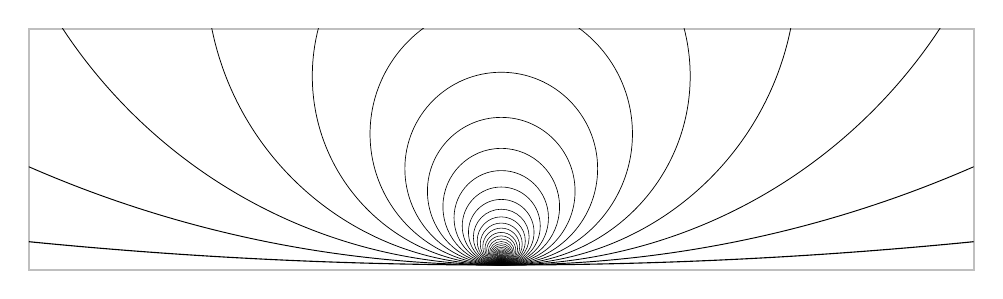
\begin{tikzpicture}[scale = 60]
		\draw[thick,lightgray] (-.1,-.001) rectangle (.1,.05);
		\clip (-.1,0) rectangle (.1,.05);
		\foreach \i in {1,...,100}{
			\draw[line width=0.4/\i^0.25 pt] (0, 1/\i^2) circle (1/\i^2);
		}
	\end{tikzpicture}
	\caption{A closeup of the Hawaiian earring $\mathbb{H}^1$.}
\end{figure}

\begin{example} \label{e:counterexample}
	Consider the \emph{$d$-dimensional Hawaiian earring}
	\begin{equation*}
		\HE = \bigcup_{n \in \N} \left\{ (x_0, \dots, x_d) \in \R^{d+1} \ \middle | \ \left( x_0 - \frac{1}{n} \right)^2 \!\! + x_1^2 + \dots + x_d^2 = \left( \frac{1}{n} \right)^2 \right\},
	\end{equation*}
	which is a compact subspace of $\R^{d+1}$.
	The function $f \colon \HE \to \R$ whose value is $0$ at the origin and is $1$ everywhere else defines a compact and weakly $\HLC$ sublevel set filtration that is not q-tame with respect to any homology theory $\H$ for which $\H_{d}(\HE)$ is infinite dimensional, as is the case for both singular and \v Cech homology.
	Specifically, using the fact that \v{C}ech homology of compact Hausdorff spaces commutes with inverse limits, it is straightforward to verify that the \v{C}ech homology in degree $d$ of the $d$-dimensional Hawaiian earring $\HE$ is isomorphic to $\prod_{n\in\N}\F$, which is infinite dimensional over $\F$.
	Moreover, the singular homology of $\HE$ is also infinite dimensional, as proven in \cite{Barratt.1962}.


	To verify that $f$ has compact sublevel sets we notice that all sublevel sets are either the empty set, the singleton containing the origin, or $\HE$ itself, all compact Hausdorff spaces.

	In order to verify that the sublevel set filtration of $f$ is weakly $\HLC$, we consider $x \in \HE$, $V$ a neighborhood of $x$ in $\HE$, and $t > f(x)$.
	We need to find a neighborhood $U \subseteq V$ of $x$ and $s \in (f(x), t)$ such that the inclusion $f_{\leq s} \cap U \hookrightarrow f_{\leq t} \cap V$ is $\HS$.
	Since we assume that $\H_{n}$ is homotopy invariant and takes singletons to finite dimensional spaces, it suffices to find $U$ as above such that $f_{\leq s} \cap U \hookrightarrow f_{\leq t} \cap V$ is homotopic to a constant map.

	If $x$ is the origin, we have $f(x) = 0$ and choose $s \in (0, \min\{t, 1\})$.
	Then $f_{\leq s} = \{x\}$, so with $U = V$ the inclusion $f_{\leq s} \cap U \hookrightarrow f_{\leq t} \cap V$ is the inclusion of $\{x\}$ into $f_{\leq t} \cap V$, which is a constant map, so the weak $\HLC$ condition is trivially satisfied.

	For $x$ different from the origin we have $f(x) = 1$ and choose $s \in (1,t)$ arbitrarily, so that $f_{\leq s} = f_{\leq t} = \HE$.
	Note that since $x$ is not the origin, there is a unique $d$-sphere in $\HE$ that contains $x$.
	Clearly, we may choose $\delta > 0$ so small that $B_{\delta}(x) = \{y \in \R^{d+1} \mid \Vert x - y \Vert < \delta\} \cap \HE$ is a topological ball contained in this sphere and contained in $V$.
	The ball $B_\delta(x)$ can be contracted to $\{x\}$ in $V$, so choosing $U = B_{\delta}(x)$, we obtain that the inclusion $f_{\leq s} \cap U \hookrightarrow f_{\leq t} \cap V$ is homotopic to the constant map with value $x$.

	It remains to be shown that $f_{\leq \bullet}$ is not q-tame for $\H$.
	This follows directly from our assumption that $\H_{d}(\HE)$ is not finite dimensional, as $f_{\leq t}$ is constant with value $\HE$ for $t \geq 1$.
\end{example}